\subsection{实验目的-了解oracle日志文件}
了解 oracle 日志文件.
%
\subsection{实验原理}
\begin{enumerate}
  \item 用户对 oracle 数据库的一切操作都记录在数据库的日志文件中,通过日志文件可以查看用户
    对数据库进行了哪些操作
  \item oracle 分三大类:
    \begin{itemize}
      \item Alert log files(告警日志)、
      \item Trace files (跟踪日志:用户和进程)
      \item redo log(重做日志:记录数据库的更改)。
    \end{itemize}
\end{enumerate}
%
\subsection{实验环境}
Windows server 2008 R2:192.168.1.3 oracle 11g
%
\subsection{实验步骤}
\subsubsection{告警日志}
告警日志文件是一类特殊的跟踪文件(trace file)。
告警日志文件命名一般为 \texttt{alert\_<SID>.log},
其中 \texttt{SID} 为 ORACLE 数据库实例名称。
数据库告警日志是按时间顺序记录 message 和错误信息。

在 ORACLE 10g 中,\texttt{BACKGROUND\_DUMP\_DEST} 参数确定了告警日志的位置,
但是告警日志的文件名无法修改。
\texttt{BACKGROUND\_DUMP\_DEST} 参数是动态的。告警日志以及所有后台跟踪文件都
会被写至 \texttt{BACKGROUND\_DUMP\_DEST} 参数所指定的目录。

在 ORACLE 11g 以及 ORACLE 12c 中,告警日志文件的位置有了变化。
主要是因为引入了 ADR
(Automatic Diagnostic Repository:一个存放数据库诊断日志、跟踪文件的目录),
关于 ADR 对应的目录位置可以通过查看 v\$diag\_info 系统视图。

在 cmd 中输入命令
\begin{minted}[bgcolor=bg,breaklines=true]{sh}
sqlplus sys/Simplexue123 as sysdba
\end{minted}
登录 oracle 数据库。
\begin{figure}[H]
  \begin{center}
    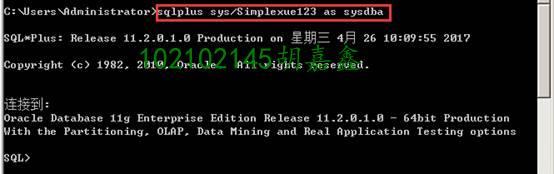
\includegraphics[width=0.40\textwidth]{2_13_1.jpeg}
  \end{center}
\end{figure}

在 SQL 中输入命令
\begin{minted}[bgcolor=bg,breaklines=true]{sql}
select * from v$diag_info;
\end{minted}
查看 ADR 对应的目录位置,可以看到 Diag Trace 对应的目录为文本格式的告警日志文件所在的目录,
而 Diag Alert 对应的目录为 XML 格式的警告日志(对应为 log.xml)。
\begin{figure}[H]
  \begin{center}
    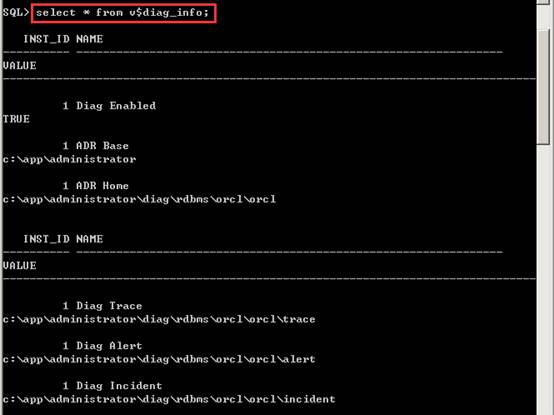
\includegraphics[width=0.40\textwidth]{2_13_2.jpeg}
  \end{center}
\end{figure}
\begin{figure}[H]
  \begin{center}
    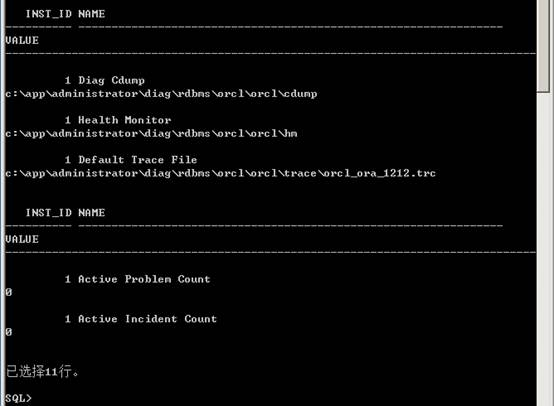
\includegraphics[width=0.40\textwidth]{2_13_3.jpeg}
  \end{center}
\end{figure}
\begin{figure}[H]
  \begin{center}
    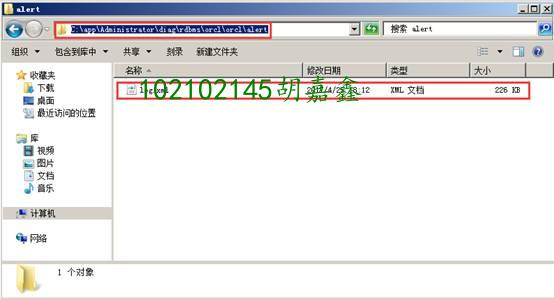
\includegraphics[width=0.40\textwidth]{2_13_4.jpeg}
  \end{center}
\end{figure}

告警日志包含了下面一些内容的信息。像一些 ORA 错误,对于监控数据库有极其重要的作用。
\begin{enumerate}
  \item 所有的内部错误(ORA-600)信息,块损坏错误(ORA-1578)信息,以及死锁错误(ORA-60)
    信息等。
  \item 管理操作,例 CREATE、ALTER、DROP 语句等,以及数据库启动、关闭以及日志归档的一些
    信息。包括以下两类:
    \begin{itemize}
      \item 涉及物理结构的所有操作:例如创建、删除、重命名数据文件与联机重做日志文件的
        \texttt{ALTER DATABASE} 命令,此外还涉及重新分配数据文件大小以及将数据文件联机与脱机的操作。
      \item 表空间操作:例如 \texttt{DROP} 与 \texttt{CREATE} 命令,
        此外还包括为了进行用户管理的备份而将表空间置入和取出热备份模式的操作
    \end{itemize}
  \item 与共享服务器或调度进程相关功能的消息和错误信息。
  \item 物化视图的自动刷新过程中出现的错误。
  \item 动态参数的修改信息。
\end{enumerate}

既然告警日志如此重要,而我们也不可能随时手工去查看告警日志文件,那么我们就必须监
控告警日志,那么监控告警日志有哪些方案呢?有以下 3 种方案:
\begin{itemize}
  \item 在 ORACLE 10g,可以将告警日志文件信息读入全局临时表,然后就可以定制一些 SQL 语句查
    询告警日志的信息。但这个方案有几个不足之处,一是如果数据库宕机了的情况下,是无
    法获取这些错误信息的,因此有些特定场景不适用。二是日志文件比较大的时候,监控告
    警日志信息比较频繁的时候,会产生不必要的 IO 操作。
  \item 通过外部表来查看告警日志文件的内容,相当的方便,与方案一一样也是使用定制
    SQL 语句来查询错误信息。
  \item 将告警日志进行归档。告警日志文件如果不加管理的话,那么文件会持续增长,有
    时候文件会变得非常大,不利于读写。一般建议将告警日志按天归档,归档文件保留三个
    月(视情况而定),可通过编写脚本来进行归档。
\end{itemize}
%
\subsubsection{跟踪日志}
跟踪文件(trace file)的作用,通常是一个服务器进程对某种异常错误条件做出响应时创
建的诊断文件。一个 sql 发到数据库,肯定会有一个
``接收请求 $\rightarrow$ 数据处理 $\rightarrow$ 返回应答''
的过程。那么就需要不同的进程来执行相应的步骤。如果进程在执行过程中发生错误,
那么就会记录到跟踪文件中。

在创建数据库的过程中遇到的错误,可以通过查找 Oracle 数据库的告警日志文件获得,
在某些情况下,还会有详细的跟踪文件生成,这些文件的位置,
在 Oracle 11g 之前,由 \texttt{*dump} 参数指定,
告警日志文件 \texttt{alert\_<ORACLE\_SID>.log} 的位置由
参数 \texttt{background\_dump\_dest} 定义。

跟踪文件的查看命令为
\begin{minted}[bgcolor=bg,breaklines=true]{sql}
show parameter SQL_TRACE;
\end{minted}
如果结果为 FALSE,
可使用命令
\begin{minted}[bgcolor=bg,breaklines=true]{sql}
alter system set SQL_TRACE = TRUE SCOPE = both;
\end{minted}
来设置打开,
使用命令
\begin{minted}[bgcolor=bg,breaklines=true]{sql}
alter system set SQL_TRACE = FALSE;
\end{minted}
来进行关闭。
\begin{figure}[H]
  \begin{center}
    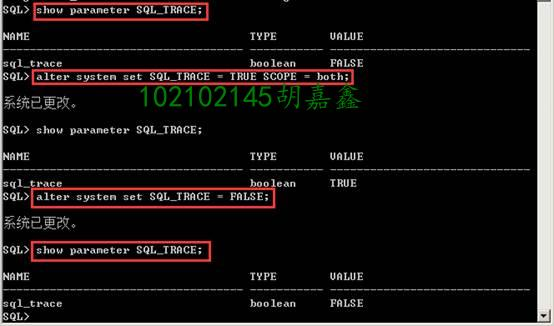
\includegraphics[width=0.40\textwidth]{2_13_5.jpeg}
  \end{center}
\end{figure}

在 SQL 中输入命令
\begin{minted}[bgcolor=bg,breaklines=true]{sql}
show parameter DUMP_DEST;
\end{minted}
查看跟踪文件位置,
会看到有三个跟踪文件目录。
\begin{figure}[H]
  \begin{center}
    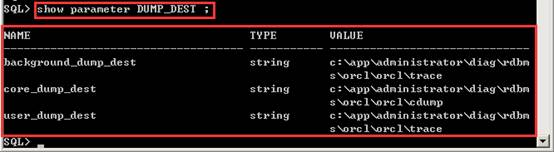
\includegraphics[width=0.40\textwidth]{2_13_6.jpeg}
  \end{center}
\end{figure}

其中,\texttt{background\_dump\_dest} 为后台转储,
\texttt{core\_dump\_dest} 为内核转储,
\texttt{user\_dump\_dest} 为用户转储,一般而言,
我们只对后台和用户转储目标感兴趣。

在 SQL 中输入命令
\begin{minted}[bgcolor=bg,breaklines=true]{sql}
show parameter background_dump_dest;
\end{minted}
查看后台转储跟踪日志文件的路径。
\begin{figure}[H]
  \begin{center}
    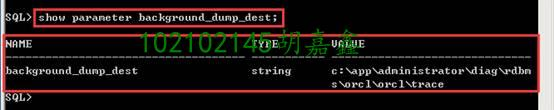
\includegraphics[width=0.40\textwidth]{2_13_7.jpeg}
  \end{center}
\end{figure}

可知跟踪日志文件所在的路径,
可以在该路径下,找到日志文件。
跟踪文件名形如:\texttt{orcl\_cjq0\_2348.trc}(SID 名+进程名+ 进程 ID)。
\begin{figure}[H]
  \begin{center}
    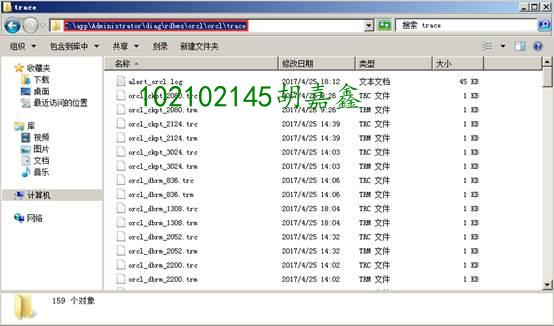
\includegraphics[width=0.40\textwidth]{2_13_8.jpeg}
  \end{center}
\end{figure}
%
\subsubsection{重做日志}
重做日志分为在线重做日志和归档重做日志。
重做日志的简单原理:
在数据更新操作 commit 前,将更改的 SQL 脚本写入重做日志。
主要用于数据库的增量备份和增量恢复。
重做日志直接对应于硬盘的重做日志文件(有在线和归档二种),重做日志文件以组(Group)
的形式组织,一个重做日志组包含一个或者多个日志文件。

online Redo log files:在线重做日志,又称联机重做日志,指 Oracle 以 SQL 脚本的形
式 实时记录数据库的数据更新,换句话说,实时保存已执行的 SQL 脚本到在线日志文件中
(按特定的格式)。

对于在线重做日志,Oracle 11g 默认对于每个数据库实例,建立 3 个在线日志组,每组一个
日志文件,文件名称为 REDO01.LOG,REDO02.LOG 和 REDO03.LOG。(用户可以通过视图操作
添加/修改/删除日志组和日志文件来自定义在线重做日志)

每组内的日志文件的内容完全相同,且保存在不同的位置,用于磁盘日志镜像,以做多次备
份提高安全性。默认情况这 3 组通常只有一组处于活动状态,不断地同步写入已操作的脚
本,当日志文件写满时(达到指定的空间配额),如果当前数据库处于归档模式,则将在
线日志归档到硬盘,成为归档日志;若当前数据库处于非归档模式,则不进行归档操作,
而当前在线日志的内容会被下一次重新写入覆盖而无法保存。因此,通常数据库在运行时,
是处于归档模式下的,以保存数据更新的日志。

当前归档日志组写满后,Oracle 会切换到下一日志组,继续写入,就这样循环切换;当处于
归档模式下,切换至原已写满的日志组,若该日志组归档完毕则覆盖写入,若没有则只能
使用日志缓冲区,等待归档完毕之后才能覆盖写入。当然,处于非归档模式下是直接覆盖
写入的。

Oracle 提供了 2 个视图用于维护在线重做日志:V\$LOG 和 V\$LOGFILE,
我们可以通过这两个视图查看和修改在线日志。

在 SQL 中输入命令
\begin{minted}[bgcolor=bg,breaklines=true]{sh}
SELECT * FROM v$log;
\end{minted}
通过 v\$log 视图查询在线日志的总体信息。
\begin{figure}[H]
  \begin{center}
    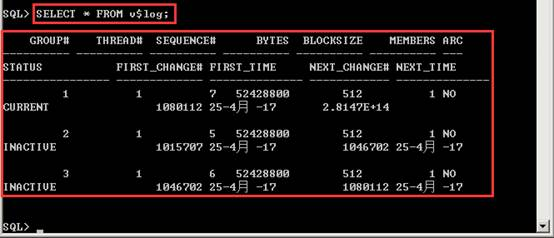
\includegraphics[width=0.40\textwidth]{2_13_9.jpeg}
  \end{center}
\end{figure}

为了便于查看,复制到 txt 文件整理后的在线日志的总体信息如下。
\begin{figure}[H]
  \begin{center}
    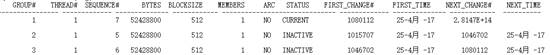
\includegraphics[width=0.40\textwidth]{2_13_10.jpeg}
  \end{center}
\end{figure}

在 SQL 中输入命令
\begin{minted}[bgcolor=bg,breaklines=true]{sql}
SELECT * FROM v$logfile ORDER BY group#;
\end{minted}
通过 v\$logfile 视图查询在线日志文件信息。
\begin{figure}[H]
  \begin{center}
    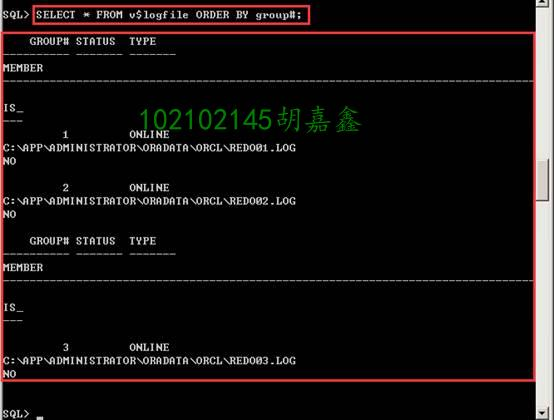
\includegraphics[width=0.40\textwidth]{2_13_11.jpeg}
  \end{center}
\end{figure}

为了便于查看,复制到 txt 文件整理后的在线日志文件信息如下。
\begin{figure}[H]
  \begin{center}
    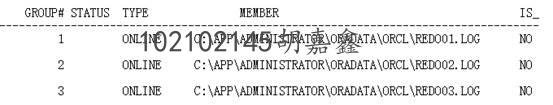
\includegraphics[width=0.40\textwidth]{2_13_12.jpeg}
  \end{center}
\end{figure}

此外可以通过 ALTER、DATABASE、ADD、DELETE 等命令增加、
修改或删除在线日志或日志组.

Archive Redo log files:归档重做日志,简称归档日志,
指当条件满足时,Oracle 将在线重做日志以文件形式保存到硬盘(持久化)。

所谓的归档,就是指将在线日志进行归档、持久化到成固定的文件到硬盘,便于以后的恢
复和查询。当然,前提条件是数据库要处于归档模式。

Oracle 11g 默认是为归档日志设定 2 个归档位置,
这 2 个归档位置的的归档日志的内容完全一致,但文件名不同。
